\section{Návrh riešenia} \label{sec_solution}
\subsection{Výber kopu na rozšírenie} \label{sec_kick}
Základom pre pokusy sú 2 symetrické kopy --- \texttt{kick\_left\_normal\_stand}, \texttt{kick\_right\_normal\_stand}, ktorých autorom je Pavol Meštaník (popis v kapitole \ref{sec_mestanik}) a použité boli v jeho diplomovej práci.
Ich popisy vravia:\\

\textit{\uv{Hráč vykoná priamy kop ľavou (pravou) nohou, kop je normálnej rýchlosti a je stabilný. Hráč sa po vykonaní kopu nevytáča.}}
\\

Práve stabilita hráča a konzistentnosť pohybu bol dôvod, prečo bol zvolený na testovanie a úpravy pomocou inverznej kinematiky a vytváraní kopu do strany. 


Pohyb sa skladá z ôsmich fáz. My sme skúmali fázu 5 tohto kopu, pretože v nej nastáva kontakt s loptou a teda kopnutie. Táto fáza je v \texttt{XML} súbore pomenovaná ako \texttt{kick\_left\_normal\_stand\_Phase3}.


\subsection{Závislosť pozície hráča od uhla smeru kopnutej lopty} \label{sec_foot_biliard}
Vykonali sme nasledujúci pokus. Predpokladali sme jav \uv{biliardovej gule} --- keď do seba narazia dve gule pod určitým uhlom, tá druhá vykoná pohyb tiež pod určitým uhlom. Predpokladali sme, že špička chodidla je pologuľa (polkruh). Situáciu zobrazuje obrázok \ref{pic_foot_biliard}.
\begin{figure}[H]
  \center
  
\includegraphics[scale=.5]{./data/foot_biliard}
  \caption{Vizualizácia smeru lopty pri rôznych umiestneniach chodidla}
  \label{pic_foot_biliard}
\end{figure}

Loptu sme umiestnili do stredu ihriska. Hráča sme postavili do takej vzdialenosti od lopty, aby bol do nej schopný kopnúť. Postupne sme menili pozíciu hráča o $10$ $cm$ dovtedy, kým sa hráč dotkol lopty ľavým chodidlom. Vznikli takto hraničné vzdialenosti z jednej aj druhej strany. Pokus sme vykonali 10-krát pre každú vzdialenosť. Vzhľadom na šum zo servera, sme do tabuľky zapísali 10 hodnôt konečnej absolútnej pozície lopty po vykonaní kopu. Súradnice sme spriemerovali a vypočítali, o aký veľký uhol $\alpha$ sa líši smer kopnutej lopty v porovnaní s priamym rovným kopom.

Situáciu zobrazuje obrázok \ref{pic_alpha}, kde $[x_{bs};y_{bs}]$ predstaje počiatočnú pozíciu lopty na ihrisku a $[x_{bs};y_{bs}]$ konečnú pozíciu lopty na ihrisku. Znamienka osí $x$ a $y$ sú označené rovnako ako sú určené súradnice na ihrisku.

\begin{figure}[H]
  \center
  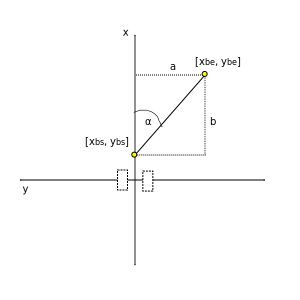
\includegraphics[scale=1]{./data/alpha}
  \caption{Uhol medzi vektorom priameho kopu a vektorom kopu do strany}
  \label{pic_alpha}
\end{figure}

Na výpočet použijeme lineárnu geometriu a dostaneme:

$$a = y_{be}-y_{bs}$$
$$b = x_{be}-x_{bs}$$
$$\tan \alpha = \frac{a}{b}$$
$$\alpha = \arctan{\frac{a}{b}} $$

Keď je lopta umiestená do stredovej pozície na ihrisku ($[0; 0]$) ako v našom prípade
$$\alpha = \arctan2(x_{be}, y_{be})$$

\begin{Definicia}
Uhlom $\alpha$ budeme nazývať uhol medzi vektorom priameho kopu a vektorom kopu do strany. 
\end{Definicia}
Ďalej budeme používať len označenie $\alpha$, prípadne \textit{alfa}.

Takto sa nám podarilo určiť, aké je postavenie hráča na ihrisku a vzdialenosť z ľavej a z pravej strany\footnote{Pre vzdialenosť ľavého chodila v jeho ťažisku platí $P_y$ + $0.055$ $m$, resp. pre pravé chodidlo  $P_y$ - $0.055$ $m$}, ak chceme dosiahnuť kopnutie do určitého smeru pod určitým uhlom. Kladné hodnoty prestavujú posun do ľavej strany a záporné do pravej.

Namerané hodnoty zobrazuje tabuľka \ref{tab_alpha}, kde $P_y$ predstavuje pozíciu hráča na osi $y$ v metroch, $\bar{\alpha_{i}}$ 
vyjadruje priemerný uhol $\alpha$ v radiánoch v pokuse $i$ pre jednu pozíciu hráča $y$ a $\bar{\alpha}$ je priemerná hodnota uhla $\alpha$ pre danú pozíciu hráča $y$ po 10 pokusov. Tabuľka zobrazuje len niektoré namerané hodnoty. Kompletná tabuľka je umiestnená na priloženom médiu v súbore \newline\texttt{experiment\_posun\_hraca.ods}.
\begin{table}[H]
\centering
\tiny
\begin{tabu}{||r||r|r|r|r|r|r|r|r|r|r||r|r||}
	\hline
	\hline
  $P_y$ & $\bar{\alpha_1}$ & $\bar{\alpha_2}$ & $\bar{\alpha_3}$ & $\bar{\alpha_4}$ & $\bar{\alpha_5}$ & $\bar{\alpha_6}$ & $\bar{\alpha_7}$ & $\bar{\alpha_8}$ & $\bar{\alpha_9}$ & $\bar{\alpha_{10}}$ & $\bar{\alpha}~(rad)$ & $\bar{\alpha}~(^{\circ})$\\
 \hline
 \hline
 $-0,113$ & $0,51$ & $0,35$ & $0,53$ & $0,53$ & $0,32$ & $0,39$ & $0,48$ & $0,37$ & $0,37$ & $0,36$ & $0,42$ & $24,21$ \\
 \hline
 $-0,11$ & $0,39$ & $0,52$ & $0,39$ & $0,5$ & $0,39$ & $0,49$ & $0,29$ & $0,32$ & $0,53$ & $0,47$ & $0,43$ & $24,62$ \\
  \hline
 $-0,1$ & $0,38$ & $0,29$ & $0,43$ & $0,32$ & $0,28$ & $0,28$ & $0,32$ & $0,31$ & $0,34$ & $0,35$ & $0,33$ & $18,92$ \\
  \hline
 $-0,09$ & $0,07$ & $0,08$ & $0,09$ & $0,06$ & $0,12$ & $0,12$ & $0,08$ & $0,09$ & $0,02$ & $0,08$ & $0,08$ & $4,62$ \\
  \hline
 $-0,08$ & $-0,1$ & $-0,12$ & $-0,14$ & $-0,11$ & $-0,13$ & $-0,12$ & $-0,12$ & $-0,13$ & $-0,11$ & $0,15$ & $-0,09$ & $-5,33$ \\
  \hline
 $-0,07$ & $-0,14$ & $-0,15$ & $-0,1$ & $-0,13$ & $-0,15$ & $-0,14$ & $-0,13$ & $-0,16$ & $-0,13$ & $-0,14$ & $-0,14$ & $-7,84$ \\
  \hline
 $-0,06$ & $-0,18$ & $-0,12$ & $-0,15$ & $-0,15$ & $-0,13$ & $-0,11$ & $-0,12$ & $-0,11$ & $-0,12$ & $-0,14$ & $-0,13$ & $-7,62$ \\
  \hline
 $-0,055$ & $-0,15$ & $-0,12$ & $-0,13$ & $-0,12$ & $-0,13$ & $-0,18$ & $-0,12$ & $-0,18$ & $-0,11$ & $-0,15$ & $-0,14$ & $-7,97$ \\
  \hline
 $-0,05$ & $-0,13$ & $-0,16$ & $-0,16$ & $-0,2$ & $-0,15$ & $-0,14$ & $-0,26$ & $-0,24$ & $-0,12$ & $-0,17$ & $-0,17$ & $-9,94$\\
  \hline
 $-0,04$ & $-0,1$ & $-0,13$ & $-0,28$ & $-0,12$ & $-0,12$ & $-0,11$ & $-0,12$ & $-0,13$ & $-0,13$ & $-0,17$ & $-0,14$ & $-8,12$ \\
  \hline
 $-0,03$ & $-0,1$ & $-0,13$ & $-0,13$ & $-0,14$ & $-0,14$ & $-0,13$ & $-0,13$ & $-0,14$ & $-0,12$ & $-0,17$ & $-0,13$ & $-7,62$ \\
  \hline
 $-0,02$ & $-0,12$ & $-0,14$ & $-0,16$ & $-0,1$ & $-0,13$ & $-0,16$ & $-0,12$ & $-0,17$ & $-0,21$ & $-0,13$ & $-0,14$ & $-8,18$ \\
  \hline
 $-0,01$ & $-0,13$ & $-0,18$ & $-0,18$ & $-0,1$ & $-0,14$ & $-0,12$ & $-0,12$ & $-0,11$ & $-0,11$ & $-0,11$ & $-0,13$ & $-7,39$\\
  \hline
 $0$ & $-0,15$ & $-0,19$ & $-0,19$ & $-0,26$ & $-0,18$ & $-0,17$ & $-0,16$ & $-0,19$ & $-0,28$ & $-0,14$ & $-0,19$ & $-10,95$ \\
  \hline
 $0,01$ & $-0,39$ & $-0,37$ & $-0,21$ & $-0,39$ & $-0,42$ & $-0,17$ & $-0,19$ & $-0,23$ & $-0,24$ & $-0,18$ & $-0,28$ & $-15,94$ \\
  \hline
 $0,02$ & $-0,18$ & $-0,36$ & $-0,62$ & $-0,48$ & $-0,48$ & $-0,54$ & $-0,54$ & $-0,38$ & $-0,44$ & $-0,51$ & $-0,45$ & $-25,96$\\
 \hline
 \hline
\end{tabu}
	\caption{Uhol alfa po vykonaní kopu posuvaním hráča po osi $y$ ihriska}
	\label{tab_alpha}
\end{table}

Ak si položíme hodnoty smeru konečnej pozície lopty na osi $x$ a posun hráča na osi $y$ ihriska na os $y$ dostaneme závislosť, ktorú zobrazuje obrázok \ref{pic_alfa_dependent_y_shift} a vyjadruje rovnica trendovej čiary \ref{eq_alfa_dependent_y_shift}. 

\begin{figure}[H]
	\centering
	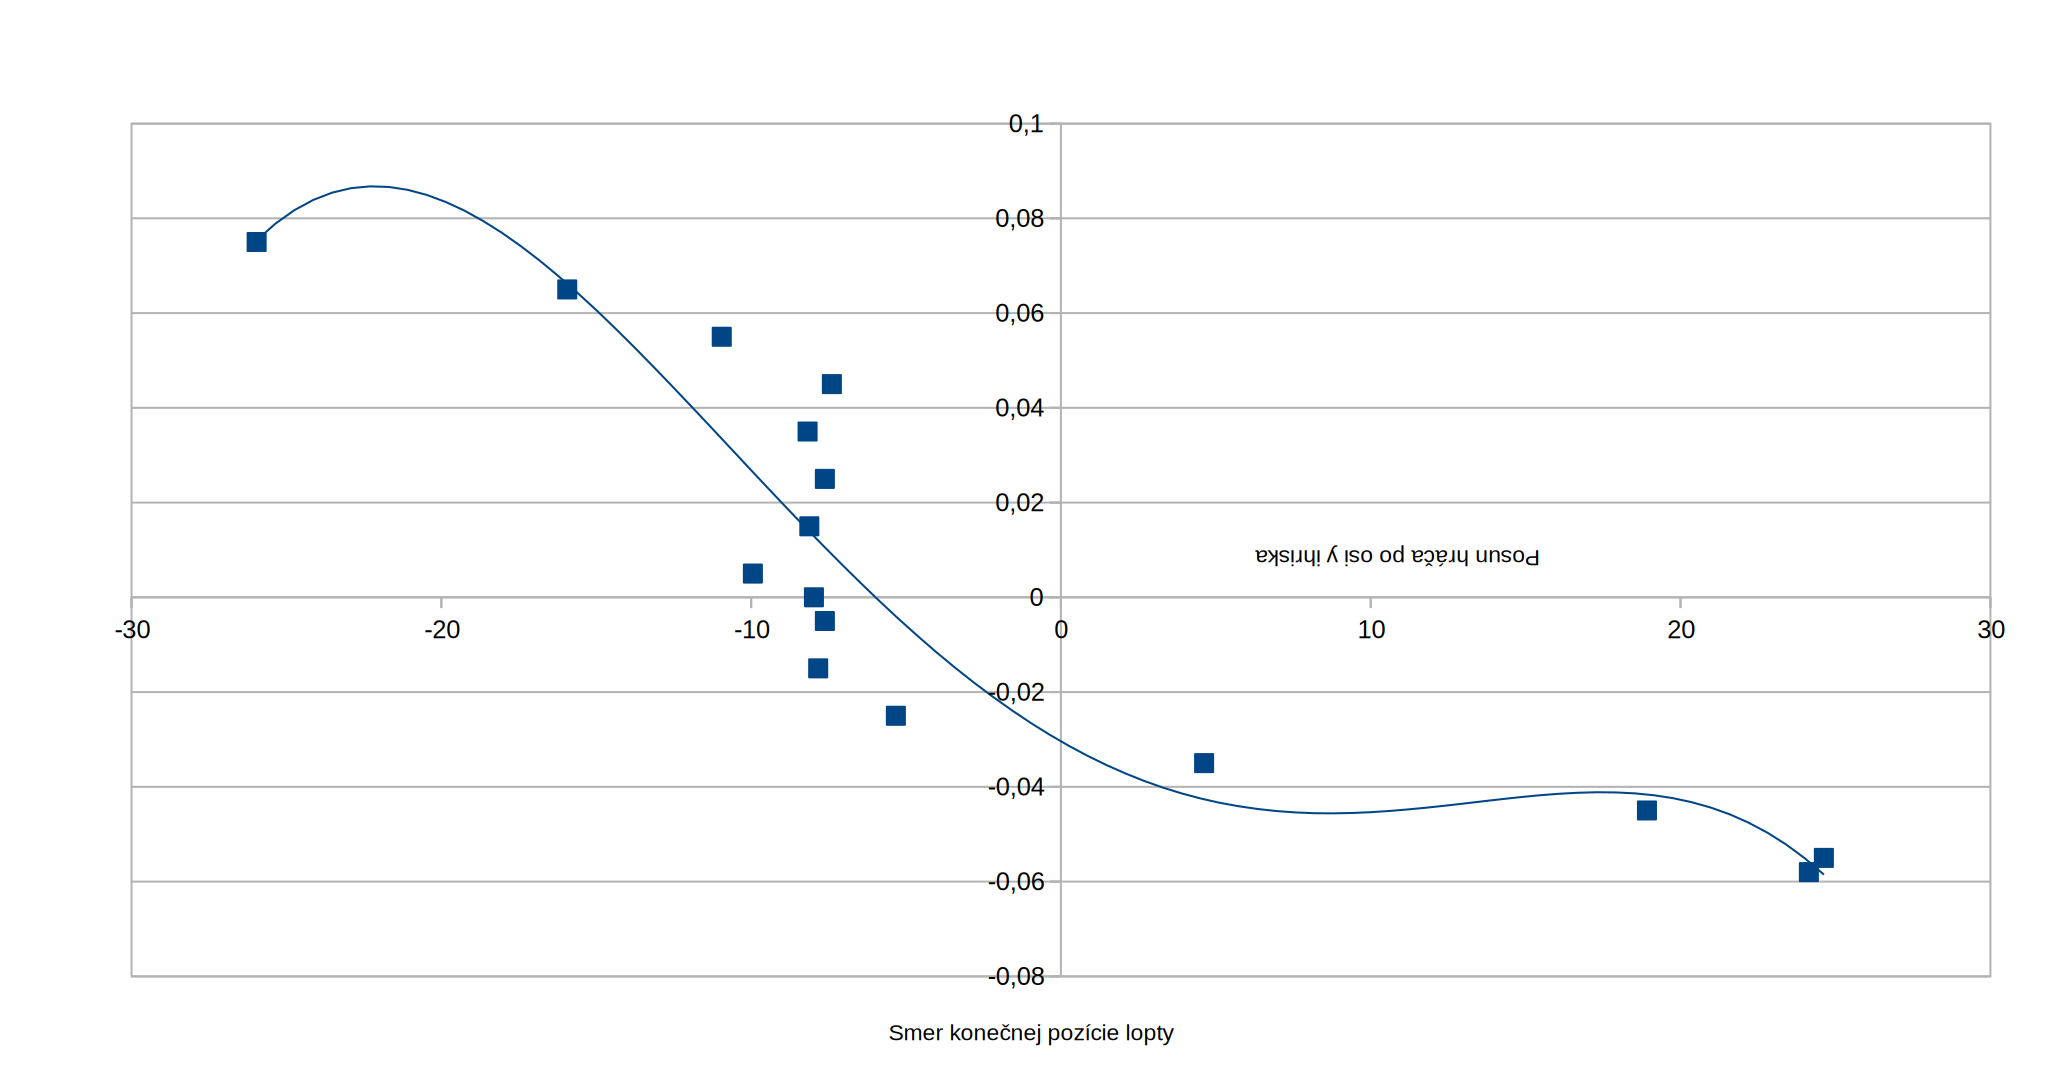
\includegraphics[scale=0.5]{./data/alfa_dependent_y_shift}
	\caption{Závislosť posunu hráča na osi $y$ ihriska od uhla alfa}
	\label{pic_alfa_dependent_y_shift}
\end{figure}

\begin{eqnarray}\label{eq_alfa_dependent_y_shift}
 f(x) =  - 2,7982597316471 \times 10^{-7}x^4 + 1,48547703927838\times 10^{-6}x^3 \\ \nonumber
 + 0,0002393458x^2 - 0,0037578029x - 0,0854023051
\end{eqnarray}

%\begin{equation} 
% f(x) =  - 2,7982597316471 \times 10^{-7}x^4 + 1,48547703927838\times 10^{-6}x^3 \\
% + 0,0002393458x^2 - 0,0037578029x - 0,0854023051
%\end{equation}

Z obrázku \ref{pic_alfa_dependent_y_shift} je možné vidieť, že hodnoty niektoré hodnoty želaného uhla $\alpha$ \uv{kazia} funkciu \ref{eq_alfa_dependent_y_shift}. Ide o hodnoty približne v intervale $<-10;-5>$ na osi $x$. Pre približne rovnaké smery lopty existujú rôzne posuny hráča. Ak tieho hodnoty odstránime z grafu, dostaneme upravený graf na obrázku \ref{pic_alfa_dependent_y_shift_updated}. Graf si rozdelíme na 2 intervaly, ktoré opisujú aproximované lineárne rovnice \ref{eq_alfa_dependent_y_shift_updated} a \ref{eq_alfa_dependent_y_shift_updated2}

\begin{figure}[H]
	\centering
	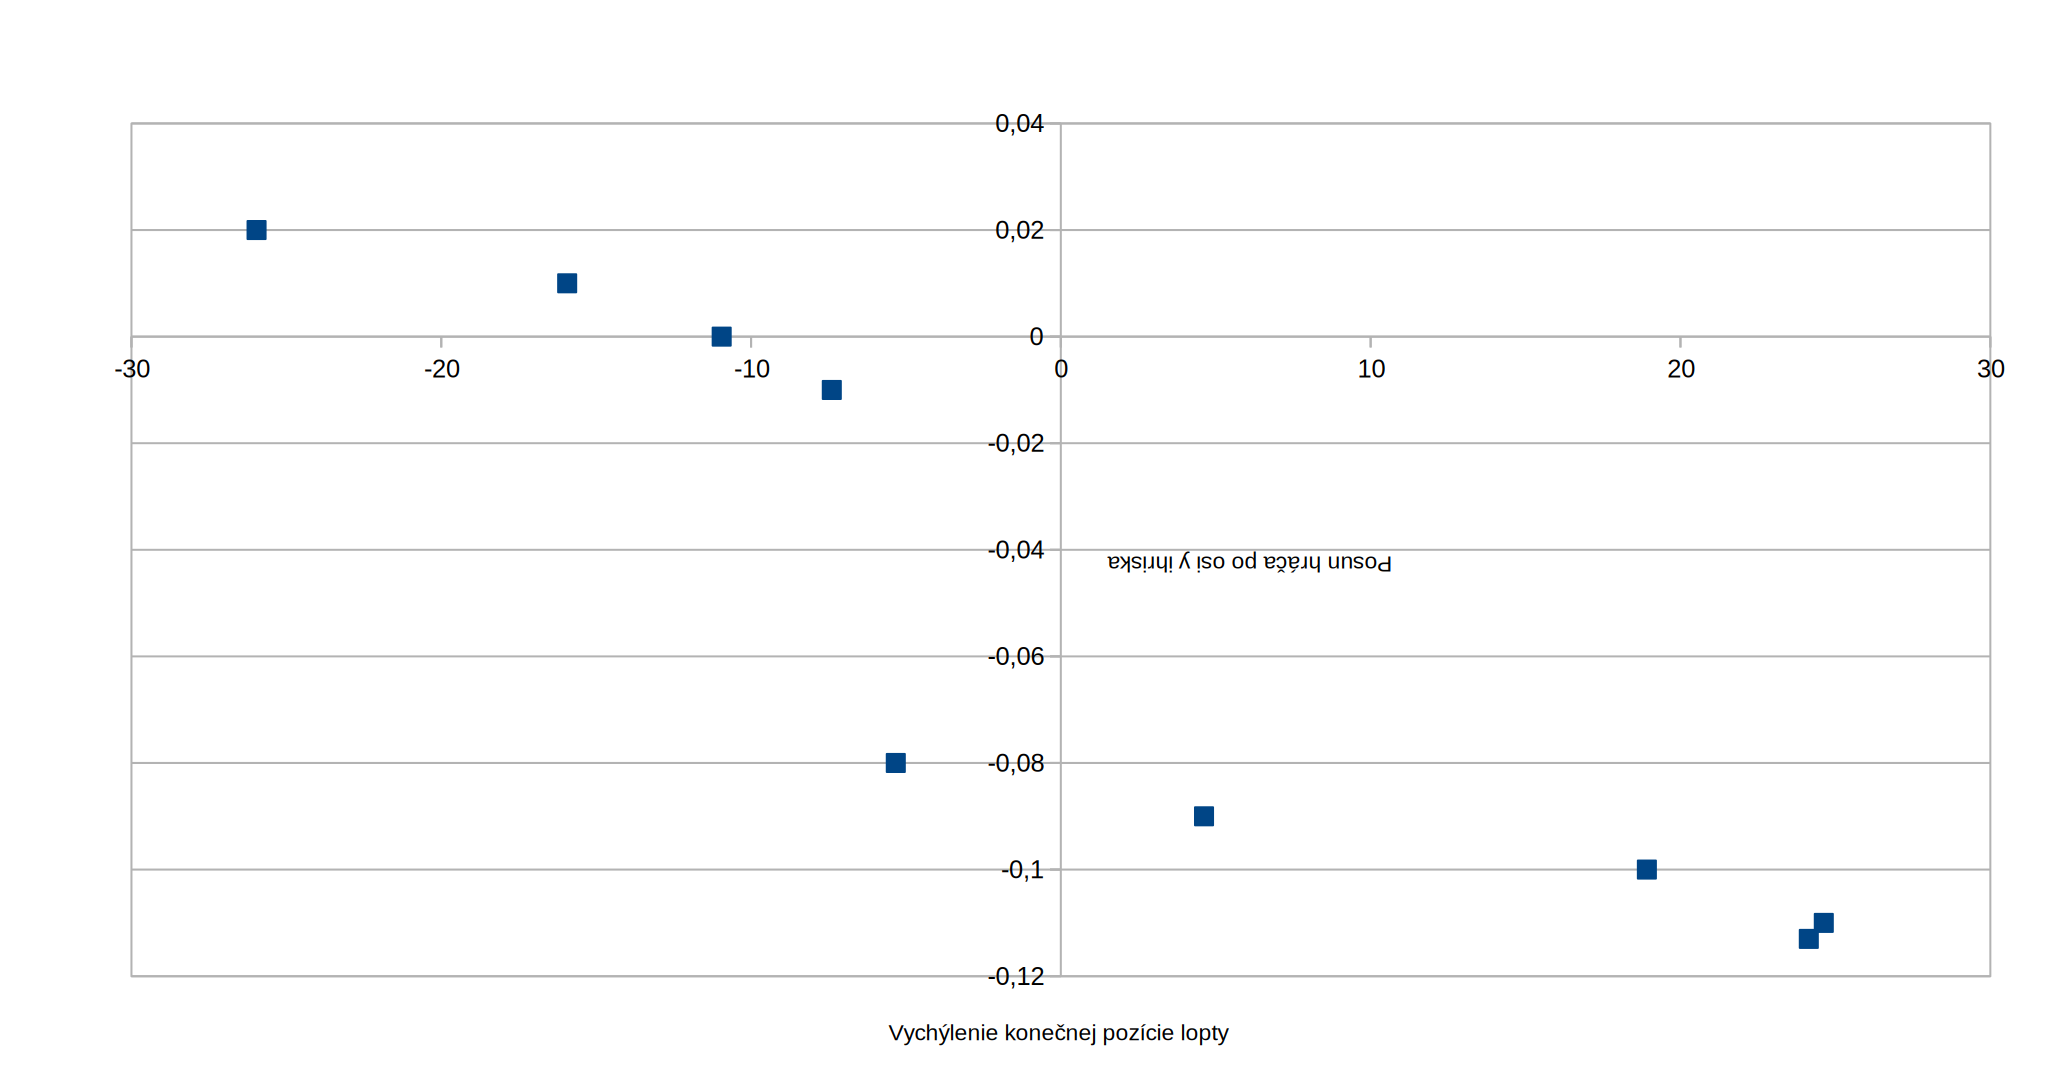
\includegraphics[scale=0.5]{./data/alfa_dependent_y_shift_updated}
	\caption{Závislosť posunu hráča na osi $y$ ihriska od uhla alfa (upravená)}
	\label{pic_alfa_dependent_y_shift_updated}
\end{figure}


\begin{equation} \label{eq_alfa_dependent_y_shift_updated}
 f(x) = -0,0015539554x - 0,018402892~~~~ x \in <-25,9;-7>
\end{equation}

\begin{equation} \label{eq_alfa_dependent_y_shift_updated2}
 f(x) = -0,001020809x - 0,0849254591 ~~~~ x \in(-7;24,6>
\end{equation}


\subsection{Závislosti natočenia kĺbu LLE2 a uhla alfa} \label{sec_lle2}
V ďalšom pokuse sme sa rozhodli skúmať závislosť natočenia kĺbu \texttt{LLE2} a uhla $\alpha$. Kĺb \texttt{LLE2} vykonáva pohyb dolnej končatiny po osi $y$ vzhľadom na základné postavenie hráča. 

Loptu sme umiestnili do stredu ihriska na pozíciu $[0;0;0]$ a hráča tak, aby stred chodidla na ľavej nohe a stred lopty ležali na osi $x$ a hráč bol schopný kopnúť ľavým chodidlom ($[-0,2; -0,055; 0,4]$ $m$). Natočenie kĺbu sme zvyšovali o $3^{\circ}$ a pre každé natočenie pokus opakovali $10$-krát. Do tabuľky zapísali 5 údajov súradníc $x$, $y$ konečnej pozície lopty. Veľkosť uhla $\alpha$ sme určili rovnako ako v predchádzajúcom experimente z kapitoly \ref{sec_foot_biliard}. 

Tabuľka \ref{tab_lle2} zobrazuje namerané hodnoty pri meniacom natočení kĺbu \texttt{LLE2}, kde $LLE2$ predstavuje natočenie kĺbu v stupňoch, $\bar{x}$ a $\bar{y}$ priemerné hodnoty konečnej pozície lopty $x$ a $y$ na ihrisku v metroch a $\alpha$ výsledný uhol smeru kopnutej lopty. Kompletná tabuľka sa nachádza na priloženom médiu v súbore (\texttt{experiment\_LLE2.ods}) spoločne s log súbormi meraní.

Ak si položíme hodnoty smeru konečnej pozície lopty na osi $x$ a natočenie kĺbu \texttt{LLE} na os $y$, dostame graf na obrázku \ref{pic_LLE2_dependency_alpha}, ktorej závislosť vyjadruje rovnica trendovej čiary \ref{eq_lle2}. 

\begin{table}[H] 
  \centering
  \begin{tabular}{||r||r|r||r|r||}
  	\hline
    \hline
   	$LLE2~(^{\circ})$ & $\bar{x}~(m)$ & $\bar{y}~(m)$ & $\bar{\alpha}~(rad)$ & $\bar{\alpha}~(^{\circ})$\\
   	\hline
   	\hline
   	$15$ & $2,71$ & $0,17$ & $0,06467$ & $3,7058$\\
   	\hline
 	$18$ & $2,10$ & $-0,15$ & $-0,0719$ & $-4,1222$ \\
 	\hline
 	$21$ & $2,06$ & $-0,22$ & $-0,1088$ & $-6,2354$ \\
 	\hline
 	$24$ & $2,02$ & $-0,31$ & $-0,1556$ & $-8,9153$ \\
 	\hline
 	$27$ & $2,02$ & $-0,34$ & $-0,1696$ & $-9,7217$ \\
 	\hline
 	$30$ & $2,06$ & $-0,39$ & $-0,1883$ & $-10,7916$\\
 	\hline
 	$33$ & $2,04$ & $-0,35$ & $-0,1686$ & $-9,6650$ \\
	 \hline
 	$36$ & $1,99$ & $-0,47$ & $-0,2339$ & $-13,4060$ \\
 	\hline
 	$39$ & $1,93$ & $-0,45$ & $-0,2285$ & $-13,0970$ \\
 	\hline
 	$42$ & $1,90$ & $-0,50$ & $-0,2594$ & $-14,8644$ \\
 	\hline
	 $45$ & $1,86$ & $-0,56$ & $-0,2954$ & $-16,9255$ \\
 	\hline
 	\hline
  \end{tabular}
  \caption{Hodnoty smeru konečnej pozície lopty a uhla $\alpha$ pri menenom natočení kĺbu \texttt{LLE2}}
  \label{tab_lle2}
\end{table}

\begin{figure}[H]
	\centering
	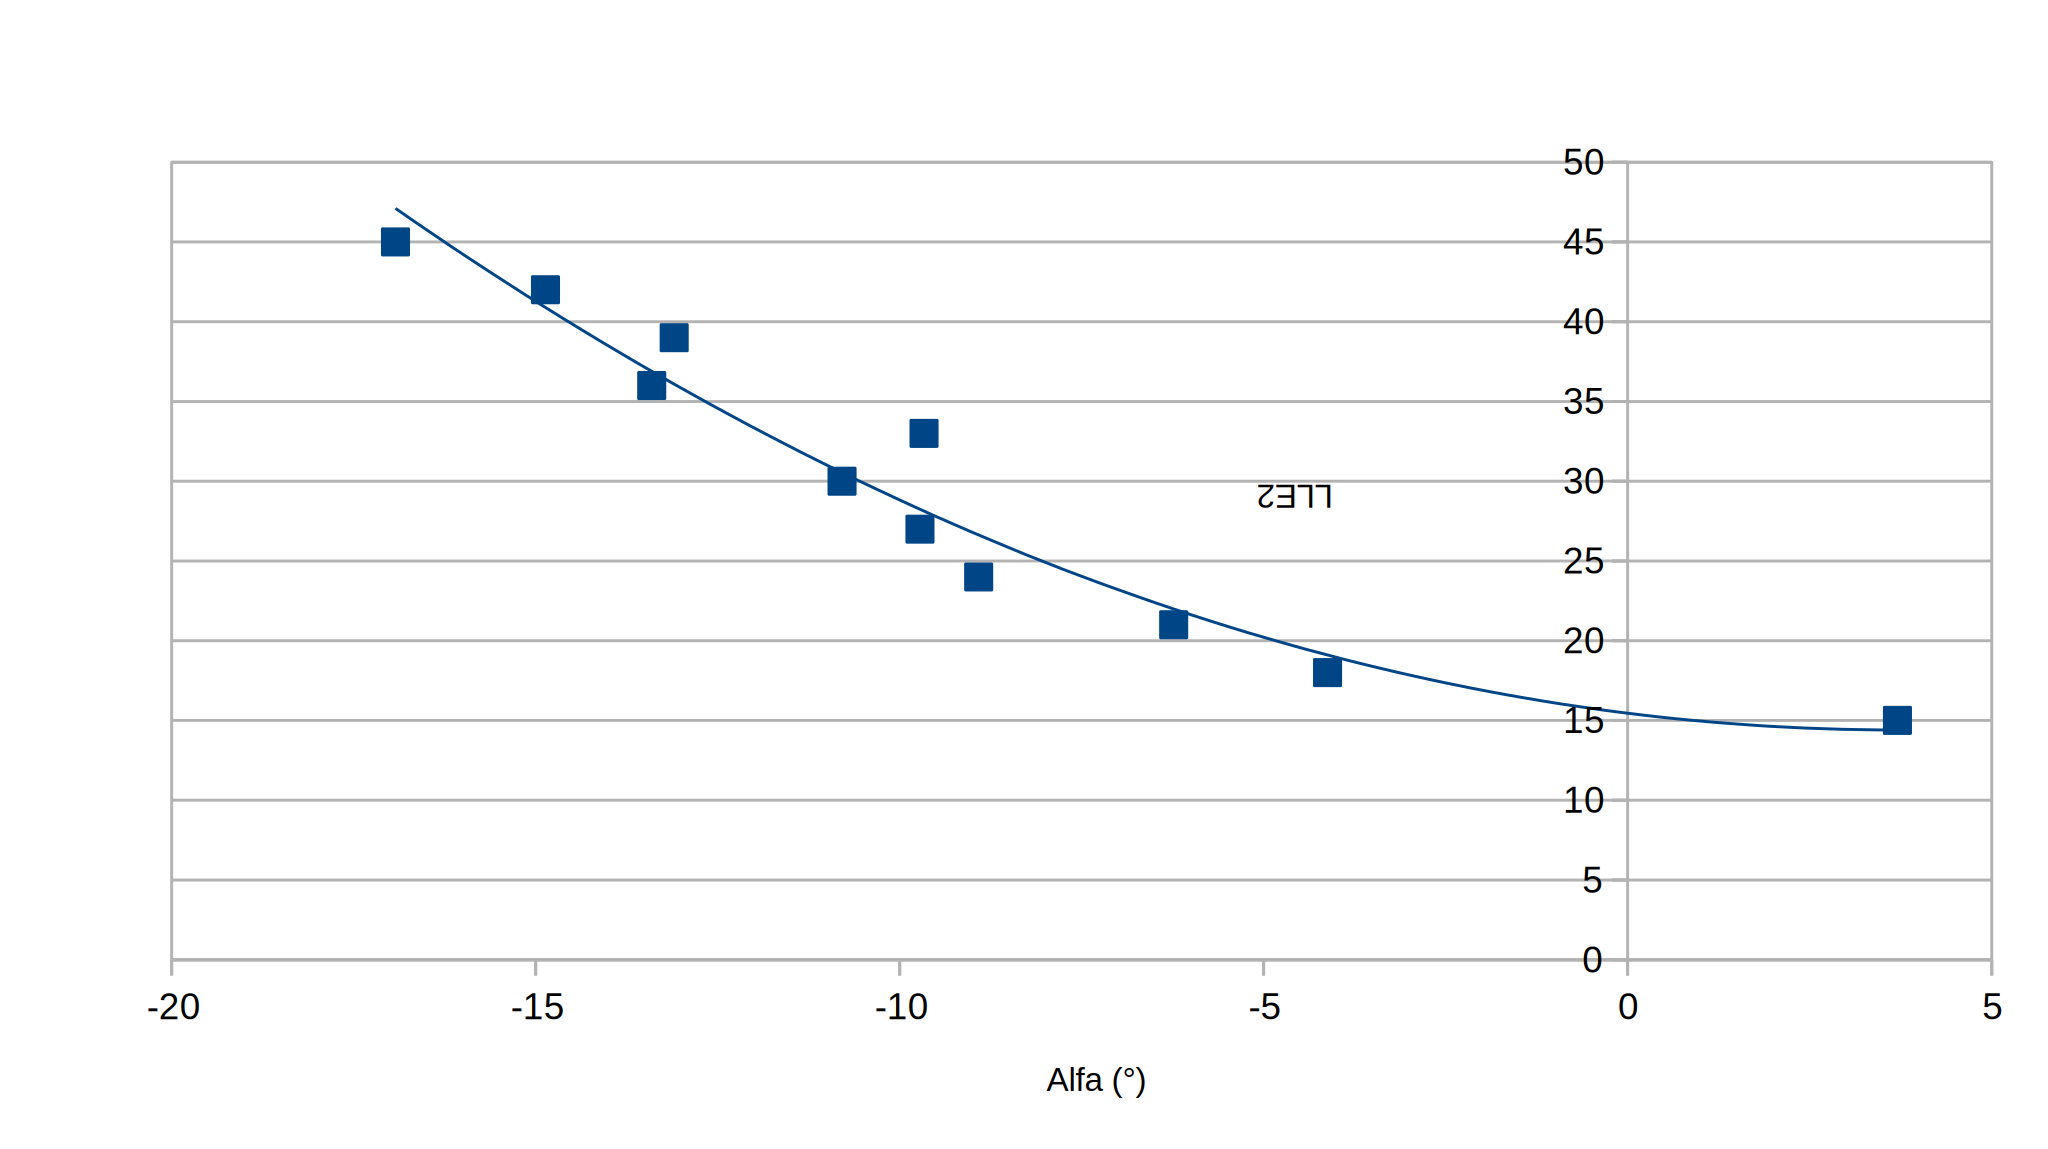
\includegraphics[scale=0.7]{./data/graf_zavislost_LLE2_od_alfa}
	\caption{Funkcia závislosti natočenia kĺbu LLE2 od uhla $\alpha$}
	\label{pic_LLE2_dependency_alpha}
\end{figure}

\begin{equation} \label{eq_lle2}
	f(x) = 0,0769165501x^2 - 0,5679788145x + 15,4529727642
\end{equation}

Pre závislosť kĺbu \texttt{RLE2} pre pravú nohu platí takáto závislosť použitím rovnice \ref{eq_lle2}, ak si $f(x)$ označíme ako $f_l(x)$

\begin{equation} \label{eq_rle2}
	f_r(x) = -f_l(x)
\end{equation}

\subsection{Závislosti natočenia kĺbu LLE6 a uhla alfa}

V ďalšom pokuse sme sa rozhodli skúmať závislosť natočenia kĺbu LLE6 a uhla $\alpha$. Určili sme rovnaké testovacie podmienky ako pri experimente v kapitole \ref{sec_lle2}.

Tento experiment nebol úspešný a hráč, aj napriek meneným hodnotám uhla \texttt{LLE6}, kopal približne rovnako, ako pri kopaní podľa \texttt{kick\_left\_normal\_stand}. Výsledky preto v práci neuvádzame, ale sú dostupné v súbore \newline\texttt{experiment\_LLE6.ods} na priloženom médiu.

\subsection{Výpočet hraničných uhlov alfa fixným nastavením LLE2 a maximálnym posunom hráča} \label{sec_max_fixed_joints}

Nasledujúci experiment opisuje výsledky merania maximálnych uhlov $\alpha$ v 2 prípadoch, ktoré zodpovedajú hraničným hodnotám pozície hráča na osi $y$ ihriska a natočeniam kĺbu \texttt{LLE2} nameraných v pokusoch z kapitoly \ref{sec_foot_biliard} a \ref{sec_lle2}. Loptu sme umiestnili do stredu ihriska. 

V prvom prípade sme hráča umiestnili na pozíciu $[-0,2; 0,02]$ a hráčovi nastavili natočenie kĺbu \texttt{LLE2} na hodnotu $45$. 

V druhom prípade sa hráč nachádza na pozícii $[-0,2; -0,11]$ a kĺb \texttt{LLE2} na hodnotu $15$. V prvom prípade sme namerali hodnotu uhla $\alpha$ približne $-55,679^{\circ}$ a v druhom prípade sa uhol $\alpha$ rovná približne $27,558^{\circ}$. 

Priebeh meraní zobrazujú tabuľky \ref{tab_max_lle2_biliard_45} a \ref{tab_max_lle2_biliard_15}. Kompletné namerané dáta sa nachádzajú na priloženom médiu v súbore \newline\texttt{experiment\_max\_uhol\_do\_strany.ods}.

\begin{table}[H]
	\centering
	\begin{tabular}{||r||r|r|r||r|r||}
	\hline
	\hline
	& $LLE2~(^{\circ})$ & $P_x~(m)$ & $P_y~(m)$ &  $\alpha~(rad)$ & $\alpha~(^{\circ})$\\
	\hline
	\hline
	$1$ & $45$ & $-0,2$ & $0,02$ & $-1,00$ & $-57,73$ \\ 
	\hline
	$2$ & $45$ & $-0,2$ & $0,02$ & $-0,95$ & $-54,67$ \\ 
	\hline
	$3$ & $45$ & $-0,2$ & $0,02$ & $-0,99$ & $-56,78$ \\ 
	\hline
	$4$ & $45$ & $-0,2$ & $0,02$ & $-0,88$ & $-50,21$ \\ 
	\hline
	$5$ & $45$ & $-0,2$ & $0,02$ & $-0,99$ & $-56,74$ \\ 
	\hline
	$6$ & $45$ & $-0,2$ & $0,02$ & $-0,98$ & $-56,05$ \\ 
	\hline
	$7$ & $45$ & $-0,2$ & $0,02$ & $-0,99$ & $-57,00$ \\ 
	\hline
	$8$ & $45$ & $-0,2$ & $0,02$ & $-0,99$ & $-55,96$ \\ 
	\hline
	$9$ & $45$ & $-0,2$ & $0,02$ & $-0,96$ & $-54,95$ \\ 
	\hline
	$10$ & $45$ & $-0,2$ & $0,02$ & $-0,99$ & $-56,70$  \\ 
	\hline
	\hline
	$\bar{\alpha}$ & & & & $-0,972$ & $-55,679$ \\
	\hline
	\hline
	\end{tabular}
	\caption{Namerané hodnoty uhla $\alpha$ pri pozícii hráča na osi $y=0,02$ a zafixovaní natočenia kĺbu \texttt{LLE2} na hodnotu $45^{\circ}$}
	\label{tab_max_lle2_biliard_45}
\end{table}

\begin{table}[H]
	\begin{tabular}{||r||r|r|r||r|r||}
	\hline
	\hline
	& $LLE2~(^{\circ})$ & $P_x~(m)$ & $P_y~(m)$ &  $\alpha~(rad)$ & $\alpha~(^{\circ})$ \\
	\hline
	\hline
	$1$ & $15$ & $-0,2$ & $-0,11$ & $0,54$ & $30,84$ \\ 
	\hline
	$2$ & $15$ & $-0,2$ & $-0,11$ & $0,47$ & $27,00$ \\ 
	\hline
	$3$ & $15$ & $-0,2$ & $-0,11$ & $0,28$ & $15,88$ \\ 
	\hline
	$4$ & $15$ & $-0,2$ & $-0,11$ & $0,58$ & $33,16$ \\ 
	\hline
	$5$ & $15$ & $-0,2$ & $-0,11$ & $0,49$ & $28,54$ \\ 
	\hline
	$6$ & $15$ & $-0,2$ & $-0,11$ & $0,43$ & $24,90$ \\ 
	\hline
	$7$ & $15$ & $-0,2$ & $-0,11$ & $0,53$ & $30,19$ \\ 
	\hline
	$8$ & $15$ & $-0,2$ & $-0,11$ & $0,46$ & $26,54$ \\ 
	\hline
	$9$ & $15$ & $-0,2$ & $-0,11$ & $0,46$ & $26,47$ \\ 
	\hline
	$10$ & $15$ & $-0,2$ & $-0,11$ & $0,56$ & $32,07$ \\ 
	\hline
	\hline
	$\bar{\alpha}$ & & & & $0,481$ & $27,558$ \\
	\hline
	\hline
	\end{tabular}
	\centering
	\caption{Namerané hodnoty uhla $\alpha$ pri pozícii hráča na osi $y=-0,11$ a zafixovaní natočenia kĺbu \texttt{LLE2} na hodnotu $15^{\circ}$}
	\label{tab_max_lle2_biliard_15}
\end{table}

\subsection{Závislosti fixovaného natočenia kĺbu \texttt{LLE2} na hodnotu 15 pri menenom posune hráča a uhla alfa} \label{sec_fix_15_shift}

V tomto experimente sme zafixovali hodnotu natočenia kĺbu \texttt{LLE2} na minimálnu hodnotu $15$ stupňov. Pri takom natočení si hráč nekopne ľavou nohou do protiľahlej dolnej končanity. Následne sme postupne posúvali hráča po osi $y$ ihriska podobne ako v pokuse popísanom kapitole \ref{sec_foot_biliard}. V experimente sme namerali hodnoty, ktorých čast zobrazuje tabuľka \ref{tab_lle2_15_y_shift}. Celá tabuľka je dostupná na priloženom médiu v súbore \texttt{experiment\_posun\_hraca\_LLE2\_fix\_15.ods}.
\begin{table}[H]
\centering
  \begin{tabular}{|r|r|r|r|}
  \hline
	 & $P_{y}~(m)$ & $\bar{\alpha}~(rad)$ & $\bar{\alpha}~(^{\circ})$ \\
 \hline 
 $1$ & $-0,1$ & $0,34$ & $19,61$ \\
 \hline 
 $2$ & $-0,09$ & $0,16$ & $8,92$ \\
 \hline
 $3$ & $-0,07$ & $0,04$ & $2,26$ \\
 \hline 
 $4$ & $-0,055$ & $0,03$ & $1,6$ \\
 \hline
 $5$ & $-0,04$ & $0,03$ & $1,42$ \\
 \hline 
 $6$ & $-0,02$ & $0,06$ & $3,14$ \\
 \hline 
 $7$ & $0$ & $-0,28$ & $-15,90$ \\
 \hline
 $8$ & $0,02$ & $-0,66$ & $-37,84$ \\
  \hline
  \end{tabular}
  \caption{Namerané hodnoty uhla $\alpha$ pri zafixovanom nastavení kĺbu \texttt{LLE2} na 15 $^{\circ}$ pri meniacom sa posune hráča na osi $y$ ihriska}
  \label{tab_lle2_15_y_shift}
\end{table}

Závislosť zobrazuje graf na obrázku \ref{pic_lle2_15_y_shift} a vyjadruje rovnica trendovej čiary \ref{eq_lle2_15_y_shift}.

\begin{figure}[H]
	\centering
	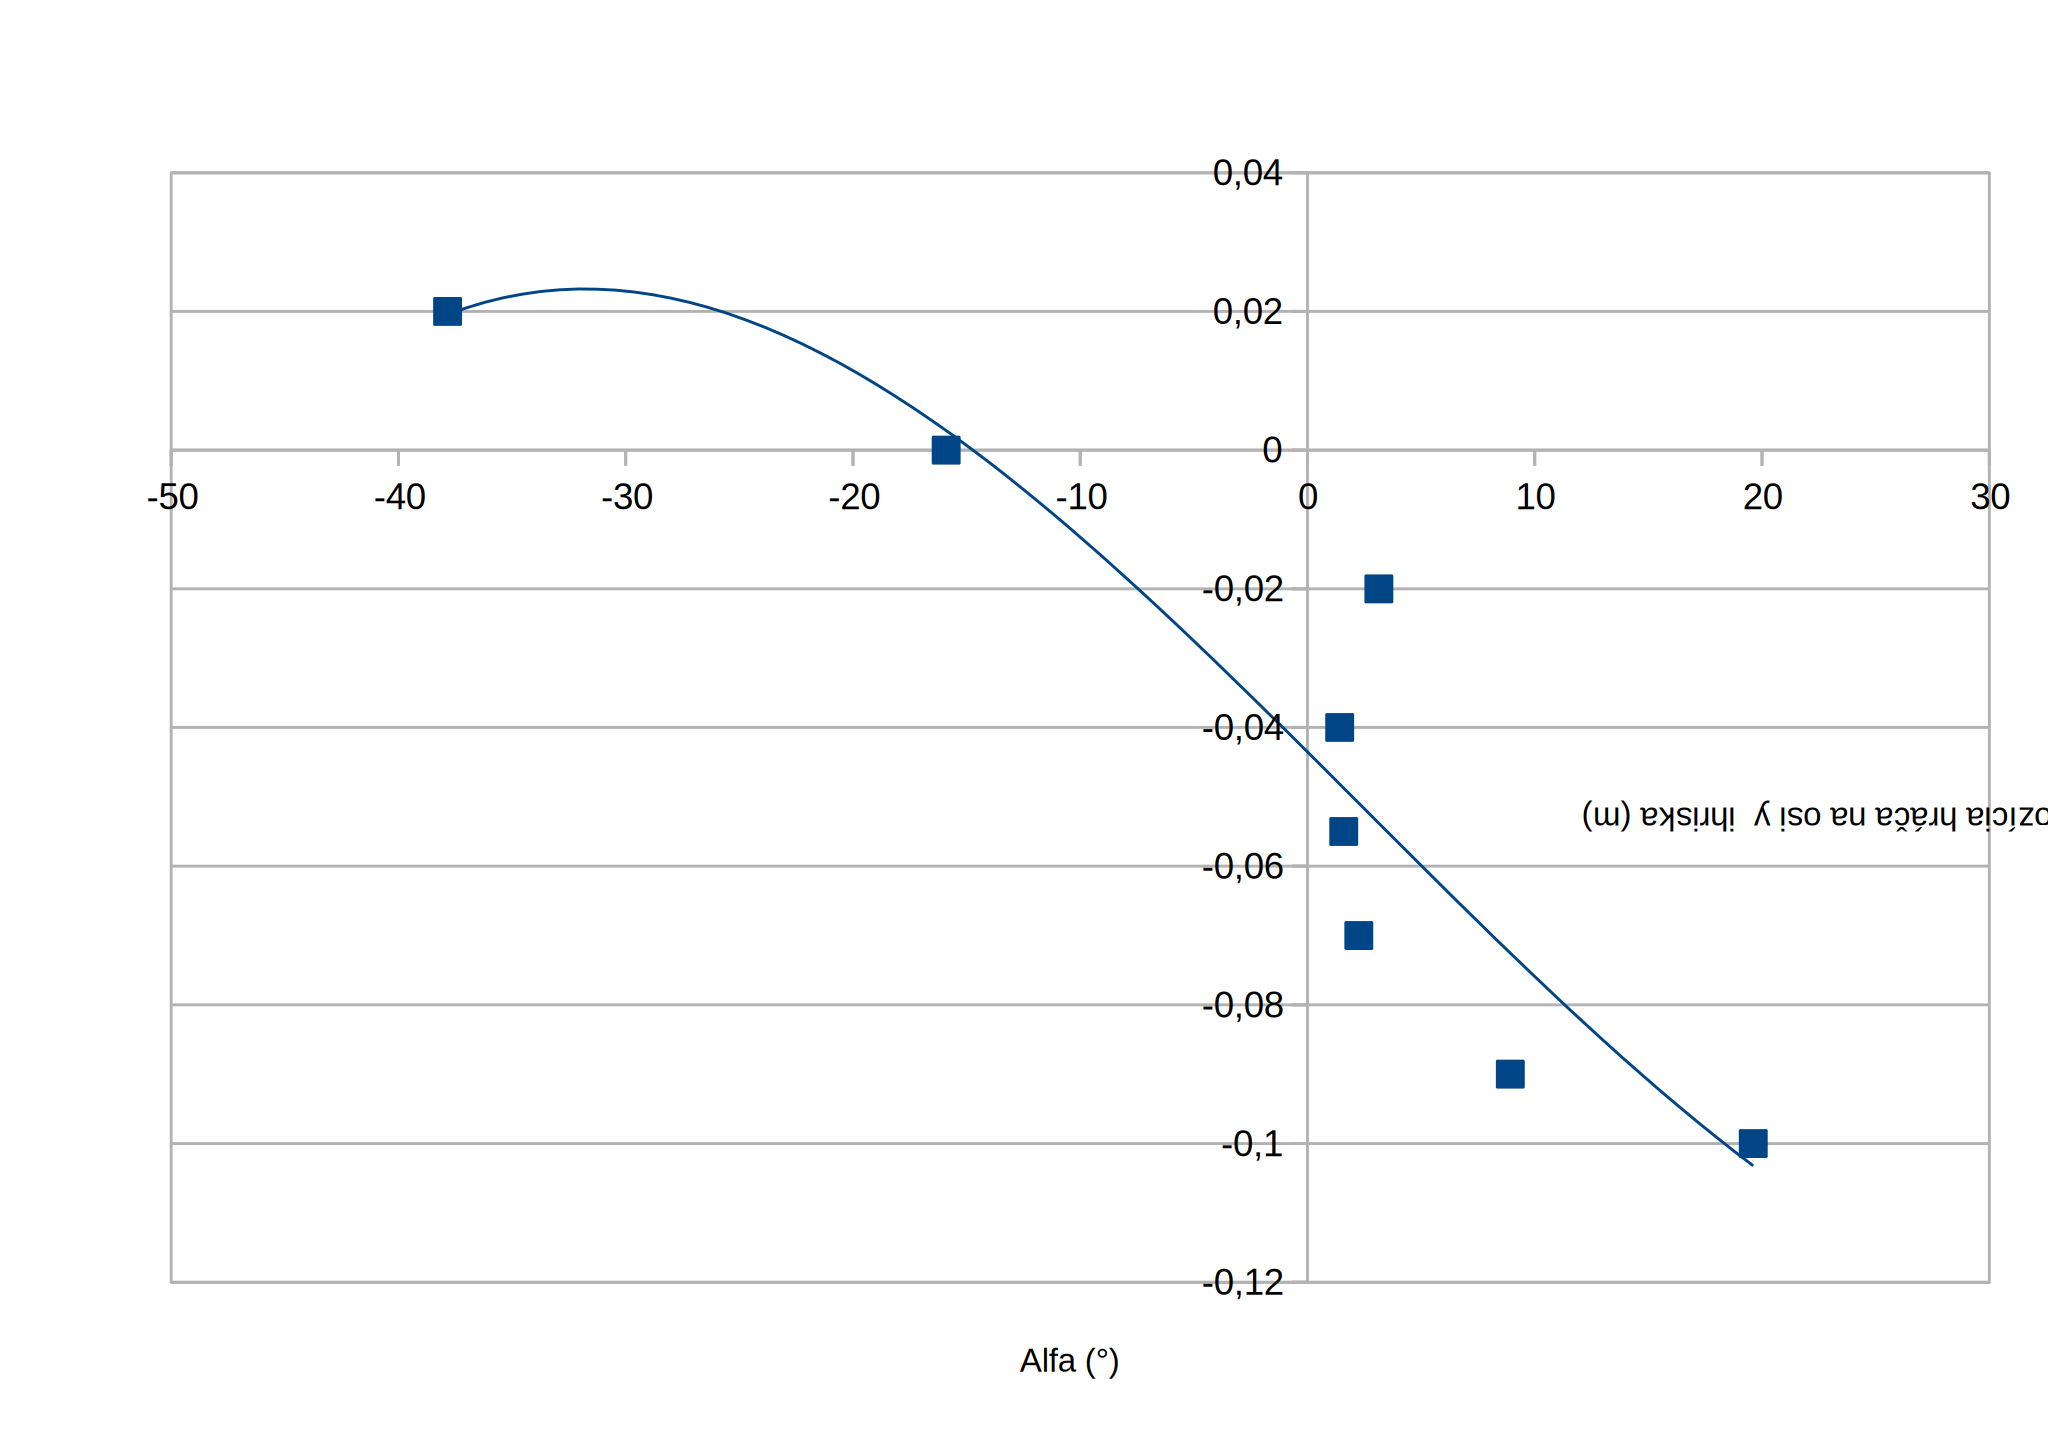
\includegraphics[scale=0.7]{./data/fixed_LLE2_15_dependency_to_shift_left}
	\caption{Závislosť pozície $y$ hráča a uhla $\alpha$ pri fixácii kĺbu \texttt{LLE2} na hodnotu $15^{\circ}$}
	\label{pic_lle2_15_y_shift}
\end{figure}

\begin{eqnarray}  \label{eq_lle2_15_y_shift}
	f(x) = 9,27342617283407\times 10^{-7}x^3 - 7,0503887961265\times 10^{-6}x^2 \\ \nonumber
	- 0,0032616022x - 0,043525855
\end{eqnarray}

\subsection{Závislosti fixovaného natočenia kĺbu \texttt{LLE2} na hodnotu 45 pri menenom posune hráča a uhla alfa} \label{sec_fix_45_shift}

V tomto experimente sme zafixovali hodnotu natočenia kĺbu \texttt{LLE2} na hodnotu 45 stupňov. Táto hodnota zodpovedá maximálnemu možnému natočeniu kĺbu \texttt{LLE2}. Následne sme posúvali hráča po osi $y$ ihriska podobne ako v pokuse popísanom kapitole \ref{sec_foot_biliard} alebo \ref{sec_fix_15_shift}. V experimente sme namerali hodnoty, ktorých časť zobrazuje tabuľka \ref{tab_lle2_45_y_shift}. Celá tabuľka je dostupná na priloženom médiu v súbore \texttt{experiment\_posun\_hraca\_LLE2\_fix\_45.ods}.

\begin{table}[H]
\centering
	\begin{tabular}{|r|r|r|r|}
	\hline
		 & $P_y~(m)$ & $\bar{\alpha}~(rad)$ & $\bar{\alpha}~(^{\circ})$ \\
	\hline
	$1$ & $-0,1$ & $-0,16$ & $-9,26$ \\
	\hline
	$2$ & $-0,09$ & $-0,27$ & $-15,42$ \\
	\hline
	$3$ & $-0,07$ & $-0,27$ & $-15,48$ \\
	\hline
	$4$ & $-0,055$ & $-0,28$ & $-15,85$ \\
	\hline
	$5$ & $-0,04$ & $-0,29$ & $-16,81$ \\
	\hline
	$6$ & $-0,02$ & $-0,34$ & $-19,53$ \\
	\hline
	$7$ & $0$ & $-0,74$ & $-42,64$ \\
	\hline
	$8$ & $0,02$ & $-0,78$ & $-44,71$ \\
	\hline
	\end{tabular}
	\caption{Namerané hodnoty uhla $\alpha$ zafixovanom nastavení kĺbu \texttt{LLE2} na $45^{\circ}$ pri meniacom sa posune hráča na osi $y$ ihriska}
	\label{tab_lle2_45_y_shift}
\end{table}

Závislosť zobrazuje graf na obrázku \ref{pic_lle2_45_y_shift} a vyjadruje rovnica trendovej čiary \ref{eq_lle2_45_y_shift}.

\begin{figure}[H]
	\centering
	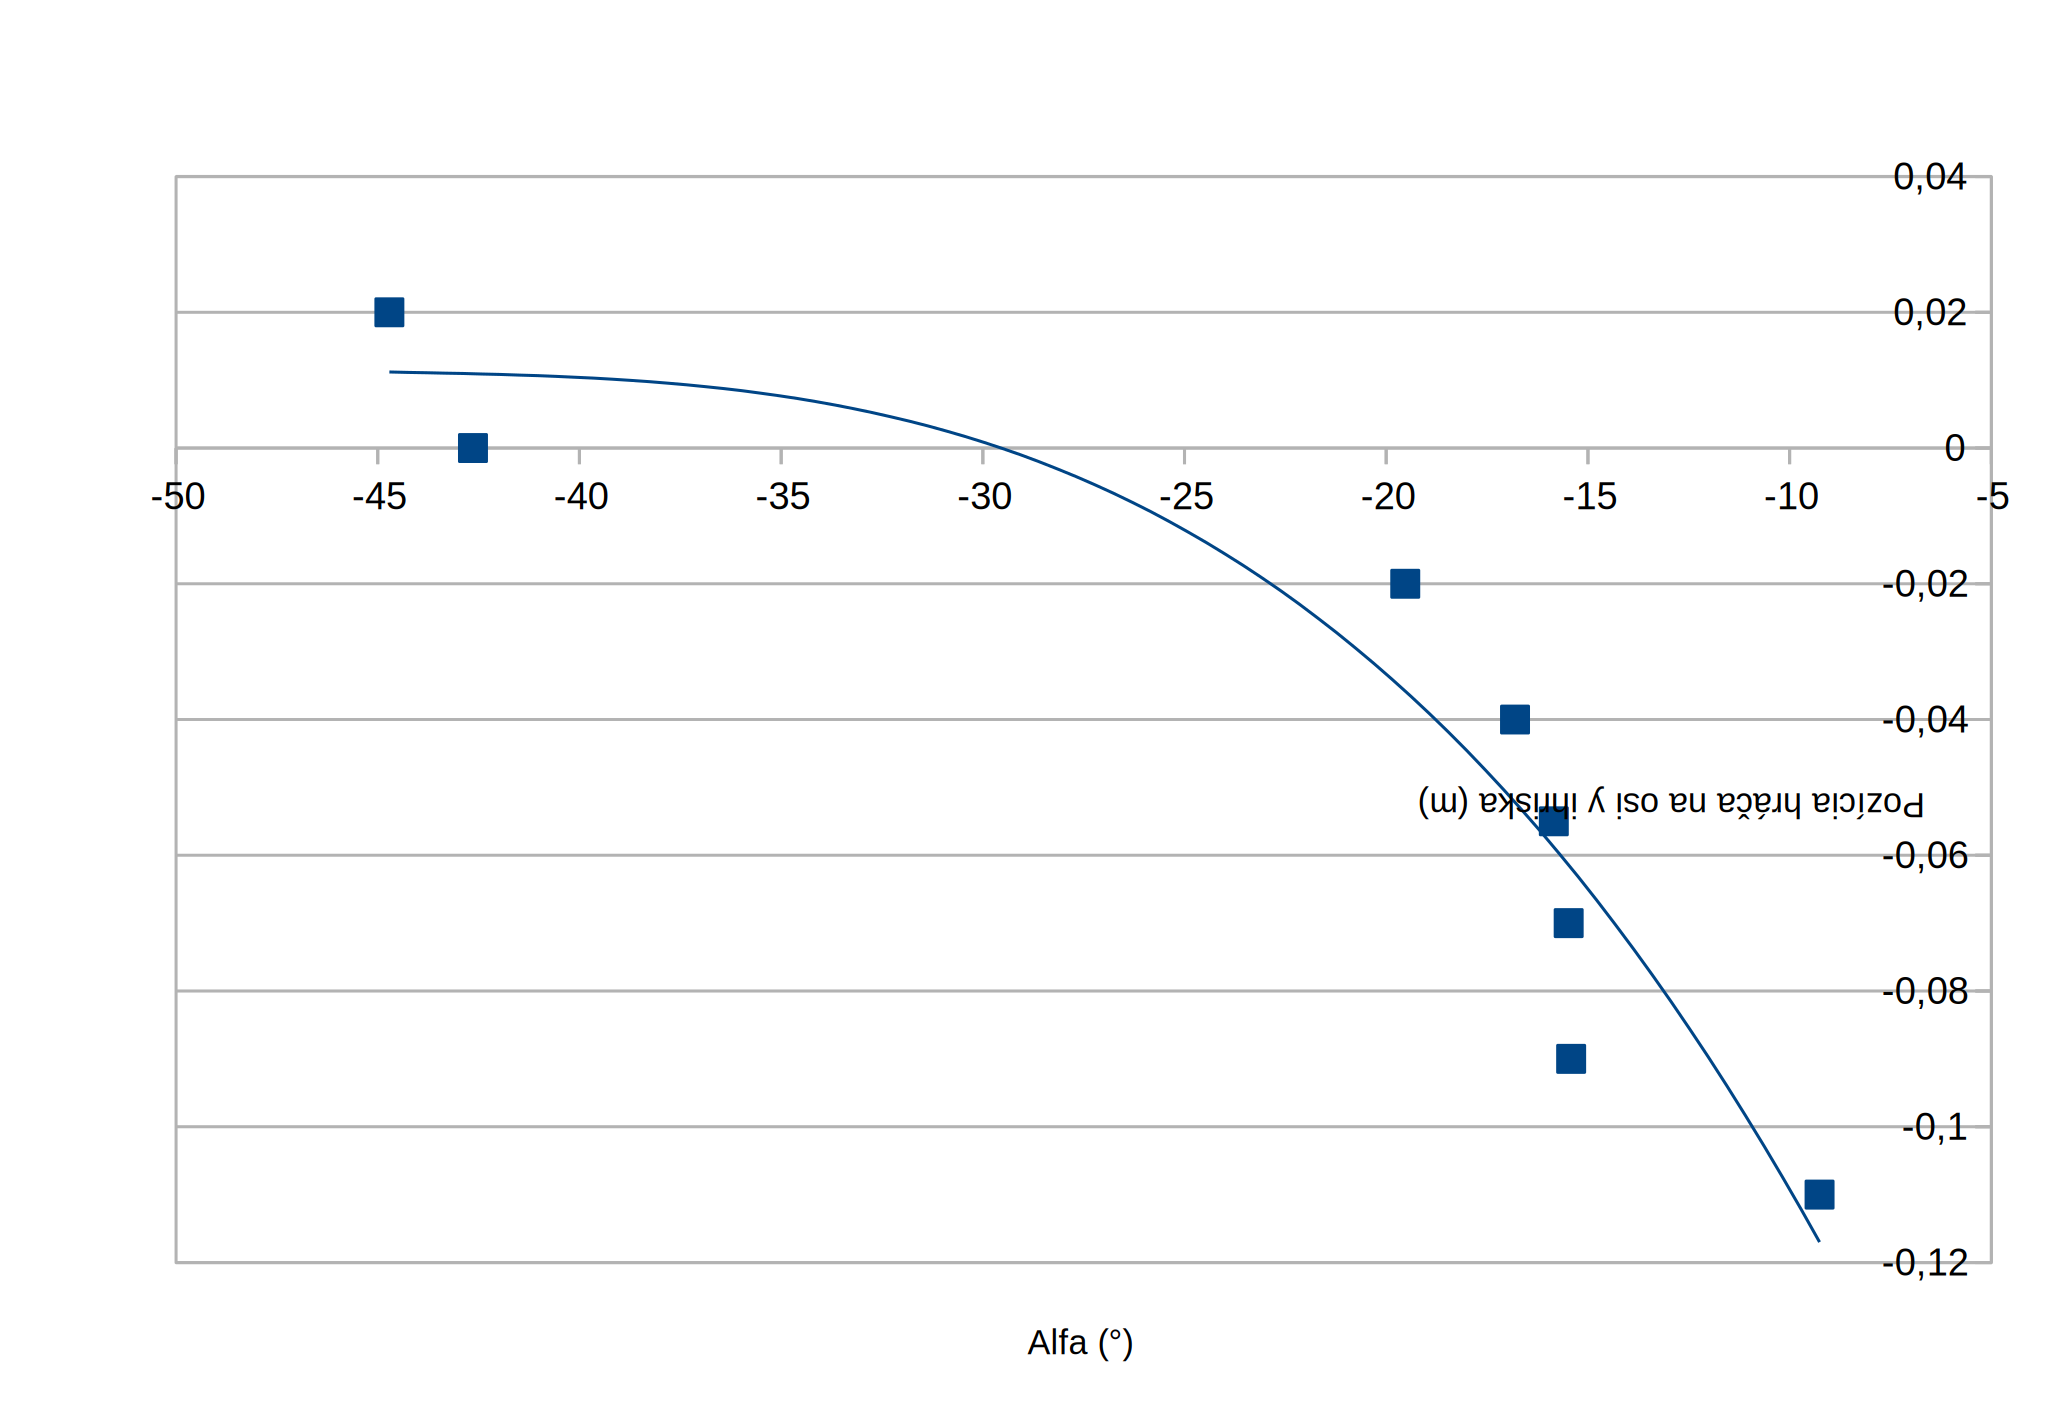
\includegraphics[scale=0.7]{./data/fixed_LLE2_45_dependency_to_shift_left}
	\caption{Závislosť pozície $y$ hráča od uhla $\alpha$ pri fixácii kĺbu \texttt{LLE2} na hodnotu $45^{\circ}$}
	\label{pic_lle2_45_y_shift}
\end{figure}

\begin{eqnarray} \label{eq_lle2_45_y_shift}
f(x) =  -2,84119818365287\times 10^{-6}x^3 - 0,0003790696x^2 \\\nonumber
- 0,0169741164x - 0,2438899745
\end{eqnarray}

